\documentclass{article}
\usepackage{lmodern}
\usepackage[T1]{fontenc}
\usepackage{array}
\usepackage{mathtools}
\usepackage{hyperref}
\usepackage{Sweave}
%\usepackage{amsmath}
\usepackage[svgnames]{xcolor}
\usepackage{listings}
%\usepackage{verbatim}
\lstset{ 
  language=R,
  numberstyle=\tiny\color{pink}
  backgroundcolor=\color{white},
  showspaces=false,
  showstringspaces=false,
  showtabs=false,
  rulecolor=\color{black},
  tabsize=2,
  captionpos=b,
  breaklines=true,
  breakatwhitespace=false,
  keywordstyle=\color{teal},      % keyword style
  commentstyle=\color{purple},   % comment style
  stringstyle=\color{orange}      % string literal style
} 

\usepackage{xcolor}
\usepackage{graphicx,subfig}
\graphicspath{ {images/} } 
%preambulo

\title{Causal inference: how to analyse causal scenarios correctly, and repercusions of a wrong analysis}
\author{Nermina Logo Lendo, Rodrigo Jiménez and Inés García Ortiz\\
      Bioinformatics and Computational Biology MSc\\
      Universidad Autónoma de Madrid\\
      2021 - 2022}
\date{January 2022}

\begin{document}
% cuerpo del documento
\maketitle
\tableofcontents
\newpage
\section{Objective}

Causal inference is a key element in statistics. It help us reach valuable conclusions about how do variables relate to one another, and help us make decisions in order to mantain our health, combat disease, adjust habits, etc. The problem comes when data is misinterpreted, and correlation is mistaken by causalty. It is very different to say 'ice cream causes cancer' rather than 'in the same season of the year, both ice cream sales and number of melanoma diagnosis increase'. A wrong conclusion can have serious repercusions, that may go from administrating a wrong treatment to ruining the ice cream economy. Even if our field of study is not statistics, it is interesting to understand some basic concepts to prevent us from being fooled by sensational news and develop the so called 'critical thinking'. 
The objective of this project is to show what changes when data is modelled in the wrong way and how to interpret it correctly. The code can be accessed from the GitHub repository \href{https://github.com/igarcia17/causal_inference}{Causalinference - GitHub repository} .
Along the document, we will explain basic concepts with examples, vaguely based in real life events. It is present all the code necessary to perform each of the cases.

\newpage

\section{What to do when there is a common cause}

In this section, we will cover the difficulties that may come when we want to analyse the cause of an outcome variable, Z, when it is affected by X. X is a variable that doesn't only affect Z, but also a second variable, Y: for this reason, X is a \textbf{common cause} of both X and Y.
We have used the following modules to make the analysis:

\begin{lstlisting}

library(dagitty)
library(car)
library(rethinking)
if(!suppressWarnings(require("rethinking", 
quietly = TRUE))) {drawdag <- plot}
  
\end{lstlisting}

The variable Y can have an effect on X or not. This gives us two basic scenarios to work on. The first scenario is illustrated in the following DAG:

\begin{lstlisting}

scenario1.DAG <- dagitty("dag {
X -> Y
X -> Z
e_y -> Y
e_z -> Z
}")

coordinates(scenario1.DAG) <- list(x = c(Y = 1, X = 2, Z = 3, e_y = 0.75, e_z = 2.75), y = c(Y = 3, X = 1, Z = 3, e_y = 2.75, e_z = 2.75))

drawdag(scenario1.DAG)

\end{lstlisting}

\begin{figure}[h]
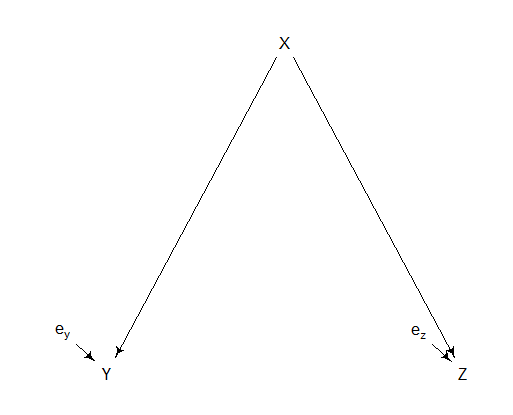
\includegraphics[width=5cm]{scenario1.DAG.png}
\centering
\end{figure}

In this first case, Y is not related to Z.
The second scenario would be:

\begin{lstlisting}
scenario2.DAG <- dagitty("dag {
X -> Y
X -> Z
Y -> Z
e_y -> Y
e_z -> Z
}")

coordinates(scenario2.DAG) <- list(x = c(Y = 1, X = 2, Z = 3, e_y = 0.75, e_z = 2.75), y = c(Y = 3, X = 1, Z = 3, e_y = 2.75, e_z = 2.75))
drawdag(scenario2.DAG)

\end{lstlisting}

\begin{figure}[h]
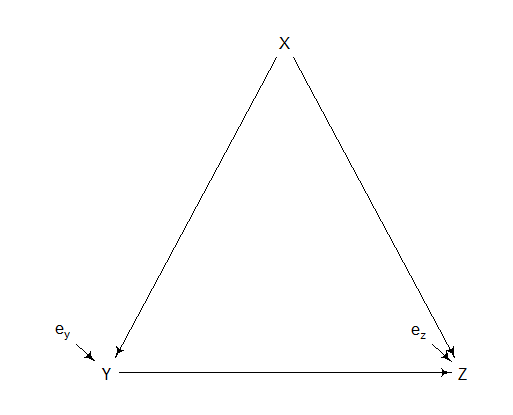
\includegraphics[width=5cm]{scenario2.DAG.png}
\centering
\end{figure}

In this second case, Y does have an effect over Z.
It is important to tell the difference between both of them, as the correct model to apply will be different. How can we tell if our data corresponds to one scenario or another?
First of all, we have to address one key problem: \textbf{how do we simulate data?}
To simulate data in different scenarios, we have used two options: vectors and a function to create datsets. To use vectors is a quick method and very versatile, but if you need to change the coefficients that relate one variable to another it is necessary to create new vectors. Meanwhile, to have a function that creates data frames is useful to make different trials in which the relation between variables is maintained and the coefficients change: the main disadvantage of this method is that anytime the structure of the DAG changes, the function is no longer valid. Both methods are valuable, and each has its advantages and disadvantages. We will use data frames in this chapter and vectors in the next one to show different ways to simulate the data.
This first function to create dataframes creates three columns: X, Y and Z. We can change the parameters that relate one varaible to another: if the estimate that multiplies Y for Z is 0, we are representing the scenario 1.

\begin{lstlisting}

create.dataset <- function(b_yz, N = 500, b_xy = 3, b_xz = 3,
                           e_x = 1, e_y = 1, e_z = 1) {
  name_df <- data.frame(X = runif(N, 1, 100) + rnorm(N, sd = e_x))
  name_df$Y <- name_df$X * b_xy + rnorm(N, sd = e_y)
  name_df$Z <- name_df$X * b_xz + name_df$Y * b_yz + rnorm(N, sd = e_z)
  return(name_df)}
Ynoinfluences <- create.dataset(0)
Yinfluences <- create.dataset(-2)
non.influences <- create.dataset(0, b_xz = 0)

\end{lstlisting}

Once this is introduce, we can go over the issue that matters. How do we know if our data belongs to scenario 1 or scenario 2?

\begin{lstlisting}
Y_check <- function (dataset, conflevel = 0.01) {
  colnames(dataset) <- c('X','Y','Z')
  model_with_Y <- lm(Z~X+Y, data = dataset)
  p.v.X <-(summary(model_with_Y)$coefficients['X','Pr(>|t|)'])
  p.v.Y <- (summary(model_with_Y)$coefficients['Y', 'Pr(>|t|)'])
  
  if ((p.v.X <= conflevel)&(p.v.Y > conflevel))
  {cat("The variable of analysis is not influenced by Y\n")
    cat('See plot\n')
    scenario1.DAG <- dagitty("dag {
    X -> Y
    X -> Z
    e_y -> Y
    e_z -> Z}")
    coordinates(scenario1.DAG) <- list(x = c(Y = 1, X = 2, Z = 3, e_y = 0.75, e_z = 2.75),y = c(Y = 3, X = 1, Z = 3, e_y = 2.75, e_z = 2.75))
    drawdag(scenario1.DAG)
    return(invisible(1))}
  
  if ((p.v.X <= conflevel)&(p.v.Y <= conflevel))
  {cat("The variable of analysis is influenced by both X and Y\n")
    cat('See plot\n')
    scenario2.DAG <- dagitty("dag {
    X -> Y
    X -> Z
    Y -> Z
    e_y -> Y
    e_z -> Z}")
    coordinates(scenario2.DAG) <- list(x = c(Y = 1, X = 2, Z = 3, e_y = 0.75, e_z = 2.75),y = c(Y = 3, X = 1, Z = 3, e_y = 2.75, e_z = 2.75))
    drawdag(scenario2.DAG)
    return(invisible(2))}

  if ((p.v.X > conflevel)&(p.v.Y > conflevel))
  {cat("It seems that neither X or Y affect Z\nYou may want to review your working model\n")
  return(invisible(0))}
  
  if ((p.v.Y <= conflevel)&(p.v.X > conflevel))
  {cat('It looks like Y is related to Z, but not Z\nYou may want to revisit the hypothesis \'X = common cause of Y and Z\'')
  return(invisible(0))}
  }
\end{lstlisting}

An example of its use is:

\begin{lstlisting}
a <- Y_check(non.influences)

## It seems that neither X or Y affect Z
## You may want to review your working model

b <- Y_check(Yinfluences)

##The variable of analysis is influenced by both X and Y
##See plot (scenario2 DAG)
\end{lstlisting}

This function could be optimized in multiple ways, but it shows that the p value of the linear model can be used to classify a data set in one scenario or another. It is necessary to have an idea beforehand of which variable may be the common cause. If by mistake Y is actually the common cause, and X is the mediator (scenario 2, but X and Y switched), the function wouldn't notice it because \textbf{this couldn't be done by p-values}. This concept, of knowing the 'structure of the DAG' or how variables are related, is crucial in causal inference, and has to be based in real facts. It is similar to which came first, the hen or the egg? Which came first, the melanoma or the exposure to UV radiation?

\section{What to do when there is a common effect}

\section{Complex cases and backdoor criteria}

\section{Conclusion}

\section{References}

\end{document}